%; whizzy chapter$B!!(B-dvi
% -initex iniptex -latex platex -format platex -bibtex jbibtex -fmt fmt
% $B0J>e(B whizzytex $B$r;HMQ$9$k>l9g$N@_Dj!#(B

%     Tokyo Debian Meeting resources
%     Copyright (C) 2012 Junichi Uekawa
%     Copyright (C) 2011 Nobuhiro Iwamatsu

%     This program is free software; you can redistribute it and/or modify
%     it under the terms of the GNU General Public License as published by
%     the Free Software Foundation; either version 2 of the License, or
%     (at your option) any later version.

%     This program is distributed in the hope that it will be useful,
%     but WITHOUT ANY WARRANTY; without even the implied warranty of
%     MERCHANTABILITY or FITNESS FOR A PARTICULAR PURPOSE.  See the
%     GNU General Public License for more details.

%     You should have received a copy of the GNU General Public License
%     along with this program; if not, write to the Free Software
%     Foundation, Inc., 51 Franklin St, Fifth Floor, Boston, MA  02110-1301 USA

%  preview (shell-command (concat "evince " (replace-regexp-in-string "tex$" "pdf"(buffer-file-name)) "&"))
% $B2hA|%U%!%$%k$r=hM}$9$k$?$a$K$O(Bebb$B$rMxMQ$7$F(Bboundingbox$B$r:n@.!#(B
%(shell-command "cd image201201; ebb *.png")

%%$B$3$3$+$i%X%C%@3+;O!#(B

\documentclass[mingoth,a4paper]{jsarticle}
\usepackage{monthlyreport}

% $BF|IU$rDj5A$9$k!"Kh7nJQ$o$j$^$9!#(B
\newcommand{\debmtgyear}{2013}
\newcommand{\debmtgmonth}{3}
\newcommand{\debmtgdate}{16}
% started from zero:
% (let ((year 2013) (month 3)) (+ (* (- year 2005) 12) month -1))
\newcommand{\debmtgnumber}{98}

\begin{document}

\begin{titlepage}
\thispagestyle{empty}
% $B%?%$%H%k%Z!<%8(B:$BJT=8I,MW$JItJ,$O:G=i$N%^%/%m$KHt$P$9$3$H(B

\vspace*{-2cm}
$BBh(B\debmtgnumber{}$B2s(B $BEl5~%(%j%"(B Debian $BJY6/2q;qNA(B\\
\hspace*{-2cm}

\includegraphics{image2012-natsu/dotdeb.pdf}\\
\hfill{}\debmtgyear{}$BG/(B\debmtgmonth{}$B7n(B\debmtgdate{}$BF|(B

% $B$3$3$O%"%C%W%G!<%H$9$k$3$H(B
% $BA43QJ8;z$K$7$J$$$H%U%)%s%H$N%5%$%:$,9g$o$J$$$N$GCm0U(B
\rotatebox{10}{\fontsize{32}{32} {\gt $BFC=8#1!'!!#X#Y#Z(B}}

\rotatebox{10}{\fontsize{32}{32} {\gt $BFC=8#2!'(B }}

\vspace*{-2cm}
\hfill{}
\includegraphics[height=6cm]{image200502/openlogo-nd.eps}
\end{titlepage}

\dancersection{Introduction}{$B>e@n(B $B=c0l(B}

\begin{multicols}{2}
 

 $B:#7n$N(BDebian$BJY6/2q$X$h$&$3$=!#$3$l$+$i(BDebian$B$N@$3&$K$"$7$rF'$_F~$l$k$H(B
 $B$$$&J}$b!"$9$G$K$I$C$W$j$H$D$+$C$F$$$k$H$$$&J}$b!"7n$K0l2s(BDebian$B$K$D$$(B
 $B$F8l$j$^$;$s$+!)(B

 Debian$BJY6/2q$NL\E*$O2<5-$G$9!#(B

 \begin{itemize}
 \item \underline{Debian Developer} ($B3+H/<T(B)$B$N0i@.!#(B
 \item $BF|K\8l$G$N!V(B\underline{$B3+H/$K4X$9$k>pJs(B}$B!W$r@0M}$7$F$^$H$a!"%"%C%W%G!<%H$9$k!#(B
 \item \underline{$B>l(B}$B$NDs6!!#(B
 \begin{itemize}
  \item $BIaCJ$P$i$P$i$J>l=j$K$$$k?M!9$,(B face-to-face $B$G=P2q$($k>l$rDs6!(B
	$B$9$k!#(B
  \item Debian $B$N$?$a$K$J$k$3$H$r8l$k>l$rDs6!$9$k!#(B
  \item Debian$B$K$D$$$F8l$k>l$rDs6!$9$k!#(B
 \end{itemize}
 \end{itemize}		

 Debian$B$NJY6/2q$H$$$&$3$H$G5f6KE*$K$O;22C<TA40w$,(BDebian Package$B$r$,$j$,$j(B
 $B$H:n$k%9!<%Q!<%O%C%+!<$K$J$C$?;Q$rLQA[$7$F$$$^$9!#>pJs$N6&M-!&3hMQ$rDL$7(B
 $B$F(B Debian$B$N:#8e$NG=F0E*$JE83+$X$NEZBf$H$7$F!"!V>l!W$H$7$F$N6u4V$rDs6!$9(B
 $B$k$N$,L\E*$G$9!#(B

$B#2#0#1#3G/$N7W2h$O2<5-$G$9!'(B
\begin{enumerate}
  \item 2013$BG/$N7W2hN)0F(B
 \item OSC $BEl5~(B nojima 
 \item UEFI$B!&%;%-%e%"%V!<%H$r(BDebian$B$G$I$&$d$k$+(B
 \item $B%;%-%e%"(BOS$B:FF~Lg(B
 \item Debian$B$G<+F02=$NL4$O8+$l$k$+(B -- $B%G!<%?%;%s%?!<$G(B OS $B$N%$%s%9%H!<%k$+$i%"%W%j$N%G%W(B
       $B%m%$!"%5!<%S%98x3+$^$G(B
 \item amazon AWS $B$G$N(B Debian $BF~Lg(B
 \item $B%9%$%9$G%-%c%s%W(B
 \item Debian $B$G%9%/%j%W%H8@8l$N%Q%C%1!<%8!'(B perl, ruby, python
 \item Debian $B$G(B apache 2.4: $B%5!<%P9=C[!"(BApache module $B%W%m%0%i%_%s%0(B
 \item Raspberry Pi $B!"(B SheevaBox$B!"(BFreedombox $B$O:#(B
 \item $B<+M3$J(BFPGA
 \item $B0lG/4V$NH?>J(B
\end{enumerate}


\end{multicols}

\newpage

\begin{minipage}[b]{0.2\hsize}
 \definecolor{titleback}{gray}{0.9}
 \colorbox{titleback}{\rotatebox{90}{\fontsize{80}{80} {\gt $B%G%S%"%sJY6/2q(B} }}
\end{minipage}
\begin{minipage}[b]{0.8\hsize}
\hrule
\vspace{2mm}
\hrule
\begin{multicols}{2}
\tableofcontents
\end{multicols}
\vspace{2mm}
\hrule
\end{minipage}

\dancersection{$B;vA02]Bj(B}{$B>e@n(B $B=c0l(B}

$B:#2s$N;vA02]Bj$O0J2<$G$9(B:
\begin{enumerate}
 \item Debian$B$G$3$3$,%P%0$C$F$k$+$b!)$H$$$&;v$K$D$$$FNs5s$/$@$5$$!#(B
 \item $B;H$C$?$3$H$N$"$k(B/$B;H$C$F$_$?$$%G%P%C%,$K$D$$$F8l$C$F2<$5$$!#(B
 \item LDAP$B$N%7%9%F%`$r4IM}$7$F$$$^$9$+!)$7$F$$$k>l9g$O!"(Bslapd.conf$B$H(Bslapd-config$B$I$A$i$r;H$C$F$$$^$9$+!)$=$NM}M3$O!)(B
\end{enumerate}
$B$3$N2]Bj$KBP$7$FDs=P$$$?$@$$$?FbMF$O0J2<$G$9!#(B
\begin{multicols}{2}
{\small
 \begin{prework}{ dictoss(杉本 典充) }

\preworksection{Debianでここがバグってるかも?という事について列挙ください。}
squeezeのvirt-manager。KVM上で動作ている仮想マシンのコンソールを操作しているとき、キーボード操作でアンダースコアが入力できない。
\preworksection{使ったことのある/使ってみたいデバッガについて語って下さい。}
gdbとpdb(python)は使ったことがあります。コマンド単独で実行するより、EmacsのGUDモード内で動作させたほうがソースコードを見つつデバッグできるので効率がいいです。(eclipseを使ったときのような感じ)。sshしつつデバッグするときはGUIがないので必要に迫られて覚えた記憶があります。
\preworksection{LDAPのシステムを管理していますか?している場合は、slapd.confと
slapd-configどちらを使っていますか?その理由は?}
LDAPシステムの管理はしたことはありません。
\end{prework}

\begin{prework}{ キタハラ }

\preworksection{Debianでここがバグってるかも?という事について列挙ください。}
 今、ぱっと思いつかない。
\preworksection{使ったことのある/使ってみたいデバッガについて語って下さい。}
 最近、prinf とか syslog 程度で済むプログラムしか作っていないなぁ。
\preworksection{LDAPのシステムを管理していますか?している場合は、slapd.confと
slapd-configどちらを使っていますか?その理由は?}
していない。(実は大昔に、Netscape の Directory Server を・・・)
\end{prework}

\begin{prework}{ まえだこうへい }

\preworksection{Debianでここがバグってるかも?という事について列挙ください。}
Debian installer では LVMを使っているとパーティション情報を削除できず、shellモードから消してましたが、今ってどうなんでしょう。

\preworksection{使ったことのある/使ってみたいデバッガについて語って下さい。}
ちょっとgdb, pdbなど使ったことありますが、ちゃんと使ったがないのでそろそろ学習せんとあかんかなぁと思ってます。
\preworksection{LDAPのシステムを管理していますか?している場合は、slapd.confと
slapd-configどちらを使っていますか?その理由は?}
今回の発表内容なので割愛
\end{prework}

\begin{prework}{ たかはしもとのぶ }

\preworksection{Debianでここがバグってるかも?という事について列挙ください。}

 うーん、あまり思いつかないです。パッケージの設定が適切でないと思うことはありますが。

\preworksection{使ったことのある/使ってみたいデバッガについて語って下さい。}
  gdb もしくは Emacs + gdb を使ったことがあります。

\preworksection{LDAPのシステムを管理していますか?している場合は、slapd.confと
slapd-configどちらを使っていますか?その理由は?}
  管理しています。ファイルベースの方が扱いやすいので、どうしてもという場合以外は slapd.conf にしています。
\end{prework}

\begin{prework}{ yamamoto }

\preworksection{Debianでここがバグってるかも?という事について列挙ください。}

\begin{description}
\item [aptitude] (armehf と ppc64 では再現しているが、他のは大丈夫みたい?)
\#659341 なのだろうが、パッチを書けるほどは理解していない。

\item [ghc] (ppc64 だけかも知れないが、確認不可。多分 7.6.1-2 の頃からだと思う)
なんか特定のパッケージの特定位置で、ビルド中に固まる。
固まった時は buildd ユーザで、ssh と gcc のゾンビプロセスがいつも残っている。

\item [libccid] 日本では結構有名な NTTCom のカードリーダに関する typo。
1.4.6 でサポートされなくなり、1.4.8 で復活したが、その時 enbug した。
最近 wheezy に上げて気づいたが、BTS しないとと思いながらも、多忙によりまだ投げられてない。
\end{description}

\preworksection{使ったことのある/使ってみたいデバッガについて語って下さい。}
バグの状況説明で gdb で bt したことがあるぐらい。

\preworksection{LDAPのシステムを管理していますか?している場合は、slapd.confと
slapd-configどちらを使っていますか?その理由は?}
LDAP って、それおいしいの?
\end{prework}

\begin{prework}{ 野島 貴英 }

\preworksection{Debianでここがバグってるかも?という事について列挙ください。}
sid/experimental使ってるとそりゃもう遭遇します(←そのためのものですから無問題ですが)。\\
今も見る例:aptitudeがLANG=ja\_JP.utf8でこける事がある(再現条件不明)、gstreamer-pluginsで字幕が使えない(upstreamの問題?)、gnome-shellがたまにハング(upstreamの問題?)、gnome-keyringがまれにハング(upstreamの問題?)などなど。ただそれでも、結局Debianの問題じゃなくて、upstreamの問題のようなものばかり...\\
※Bug報告しろよという話もある。
\preworksection{使ったことのある/使ってみたいデバッガについて語って下さい。}
printf(笑)/gdb/perldb/pydb/adb/apd/xdebugなどなど。
\preworksection{LDAPのシステムを管理していますか?している場合は、slapd.confと
slapd-configどちらを使っていますか?その理由は?}
 秘密。slapd.conf直接編集かな。\\
理由:そんなに変更しないので、他の手段を使ってないだけだったりという消極的理由。
\end{prework}

\begin{prework}{ koedoyoshida }

\preworksection{Debianでここがバグってるかも?という事について列挙ください。}
debugイメージが標準で提供されていないこと。

\preworksection{使ったことのある/使ってみたいデバッガについて語って下さい。}
\begin{description}
\item [→使ったことがある] crash,lkst,gdb
\item [→使ってみたい] VisualStudio並みにグラフィカルなデバッグ環境
\end{description}
\preworksection{LDAPのシステムを管理していますか?している場合は、slapd.confと
slapd-configどちらを使っていますか?その理由は?}
過去の遺産のslapd.confのシステムが...
\end{prework}

\begin{prework}{ 鈴木崇文 }

\preworksection{Debianでここがバグってるかも?という事について列挙ください。}
あまりバグってると感じたことはないです。
\preworksection{使ったことのある/使ってみたいデバッガについて語って下さい。}
 gdbを使用したことがあります。emacs+gdbで使いやすい環境を作れたら使ってみたいです。統合開発環境としてのemacs+gdb連携ベストプラクティス的なものに興味があります。vim+gdbも試したことがありますが、結局gdbを直接使うようになってしまいました。
\preworksection{LDAPのシステムを管理していますか?している場合は、slapd.confと
slapd-configどちらを使っていますか?その理由は?}
LDAP使ったことないですね。
\end{prework}

}
\end{multicols}

\dancersection{Debian Trivia Quiz}{$B>e@n=c0l(B}

$B$H$3$m$G!"$_$J$5$s(B Debian $B4XO"$NOCBj$K$*$$$D$$$F$$$^$9$+!)(BDebian$B4XO"$NOC(B
$BBj$O%a!<%j%s%0%j%9%H$r$h$s$G$$$k$HDI@W$G$-$^$9!#$?$@$h$s$G$$$k$@$1$G$O$O(B
$B$j$"$$$,$J$$$N$G!"M}2rEY$N%F%9%H$r$7$^$9!#FC$K0l?M$@$1$G$O0UL#$,$o$+$i$J(B
$B$$$H$3$m$b$"$k$+$bCN$l$^$;$s!#$_$s$J$G0l=o$KFI$s$G$_$^$7$g$&!#(B

$B:#2s$N=PBjHO0O$O(B\url{debian-devel-announce@lists.debian.org} $B$d(B \url{debian-devel@lists.debian.org}$B$KEj9F$5$l$?(B
$BFbMF$H(BDebian Project News$B$+$i$G$9!#(B

\begin{multicols}{2}
% %; whizzy-master ../debianmeetingresume201211.tex
% $B0J>e$N@_Dj$r$7$F$$$k$?$a!"$3$N%U%!%$%k$G(B M-x whizzytex $B$9$k$H!"(Bwhizzytex$B$,MxMQ$G$-$^$9!#(B
%

\santaku
{DebConf13 $B$N3+:ECO$H3+:EF|$O!)(B}
{$BF|K\!"El5~ET(B 6$B7n(B20$BF|(B}
{$B%K%+%i%0%"(B $B%^%J%0%"(B 7$B7n(B8-14$BF|(B}
{$B%9%$%9!"%t%)!<%^%k%-%e(B 8$B7n(B11-18$BF|(B}
{3}
{$B%K%+%i%0%"$O(BDebConf12$B$N3+:ECO$G$9!#(B
DebConf13$B$O%9%$%9$N%-%c%s%WCO$G3+:E$G$9!#(B
6/20$B$O3'$5$sM=Dj$r6u$1$F$*$-$^$7$g$&!#(B}

\santaku
{$B@$3&$N(BWeb$B%5!<%P$G:G$b?M5$$N$"$k(BLinux $B%G%#%9%H%j%S%e!<%7%g%s(B(W3Techs$BD4$Y(B)$B$O!)(B}
{CentOS}
{Debian}
{Ubuntu}
{B}
{\url{http://w3techs.com/technologies/history_details/os-linux}$B$K7k2L$N%0%i%U$,$"$j$^$9!#(B
$B8=:_(B Linux $B$r;HMQ$7$F$$$k(B web $B%5!<%P$N(B 32.9\% $B$,(B Debian $B$rMxMQ$7$F$*$j!"$=$N3d9g$O8=:_$bA}2C$rB3$1$F$$$k$=$&$G$9!#(B}

\santaku
{Debian $B%+!<%M%k%A!<%`$N%a%s%P!<$G$"$j!"(Bkernel.org $B$N(B 3.2.y $B0BDjHG7ONs$N%a%s%F%J$G$b$"$k(B Ben Hutchings $B$5$s$,<!4|(B Debian $B0BDjHG$H0l=o$K=P2Y$5$l$k(B Linux $B%+!<%M%k$K(B (3.2 $B7ONs$N(B mainline $B$K$OL5$$(B) $BDI2C5!G=$,Ek:\$5$l$kM=Dj$G$"$k$H=R$Y$F$$$^$9!#(B
$BB?$/$NDI2CE@$NCf$K4^$^$l$J$$$b$N$O2?!)(B}
{PREEMPT\_RT}
{Hyper-V guest drivers$B$N6/2=(B}
{ARM64/AArch64$B%"!<%-%F%/%A%c%5%]!<%H(B}
{C}
{Hyper-V guest drivers$B$O(Bmainline kernel$B$G(B3.2$B$K$b4^$^$l$F$$$^$9$,!"$h$j2~A1$5$l$?(B3.4$B$+$i$N=$@5$,F3F~$5$l$^$9!#(B
PREEMPT\_RT$B$O%O!<%I%j%"%k%?%$%`$r<B8=$9$k$?$a$N(BPatch$B!"(B
linux-image-rt-amd64 , linux-image-rt-686-pae $B$N(Bmetapackage$B$G;HMQ$G$-$^$9!#(B
$B?7$7$$(BARM 64$B%S%C%H%"!<%-%F%/%A%c%5%]!<%H$O(Bmainline kernel 3.7$B$+$i(B}

\santaku
{Wookey$B$5$s$,%"%J%&%s%9$7$?(Balpha$BHG$N(BDebian port arm64 image$B$O!)(B}
{Debian/Ubuntu port image}
{Debian/KFreeBSD port image}
{Debian/GnuHurd port image}
{A}
{self-bootstrapp(non x86)$BBP1~$H$N$3$H$G$9!#(B\url{http://wiki.debian.org/Arm64Port}$B$G%9%F!<%?%9$,3NG'$G$-$^$9!#(B}

\santaku
{700,000$BHVL\$N%P%0$,Js9p$5$l$?F|$rEv$F$k(B700000thBugContest$B$N7k2L$,=P$^$7$?!#$=$NM=A[F|$HJs9pF|$O!)(B}
{2012/12/12$B$rM=A[$7$?(BDavidPrevot}
{$BM=A[F|(B:2013/02/04$B!"Js9pF|(B:2013/02/14}
{$BM=A[F|(B:2013/02/07$B!"Js9pF|(B:2013/02/14}
{$BM=A[F|(B:2013/02/14$B!"Js9pF|(B:2013/02/07}
{C}
{$B:G$b6a$$(B2013/02/14$B$rM=A[$7$?(BChristian Perrier$B$5$s$,Ev$F$^$7$?!#7k2L$O(B\url{http://wiki.debian.org/700000thBugContest}$B$G8x3+$5$l$F$$$^$9!#(B
$B$^$?!"(B800,000/1,000,000$BHVL\$N%P%0$,Js9p$5$l$kF|$rEv$F$k%3%s%F%9%H(B\url{http://wiki.debian.org/800000thBugContest}$B$b3+:E$5$l$F$$$^$9!#(B}

\santaku
{master.debian.org$B$,?7$7$$5!3#$K0\9T$5$l$^$7$?!#$3$l$O2?$N%5!<%P$G$7$g$&$+(B $B!)(B}
{@debian.org$B$N%a!<%k%5!<%P(B}
{$B%Q%C%1!<%8$N%^%9%?!<%5!<%P(B}
{$B%Q%C%1!<%8$N%9%]%s%5!<(B(mentor)$B$rC5$9%5!<%P(B}
{A}
{$B8E$$%5!<%P$O%G%#%9%/>c32Ey$,$"$C$?$N$G!"<wL?$HH=CG$5$l!"%G!<%?$,B;<:$9$kA0$K?7$7$$%5!<%P$K0\9T$5$l$^$7$?!#(Bftp-master.debian.org$B$O(BDebian$B$N(B official package $B%j%]%8%H%j$G$9!#%Q%C%1!<%8$N%9%]%s%5!<(B(mentor)$B$rC5$9$N$O(Bmentors.debian.net$B!#(B }

\santaku
{pbuilder$B$K(Bclang support$B$,DI2C$5$l$^$7$?!#C/$,=q$$$?%Q%C%A$G$7$g$&$+!)(B}
{Sylvestre Ledru}
{Junichi Uekawa}
{Hideki Yamane}
{C}
{Debian$B$N(BClang$B%5%]!<%H$OCe!9$H?J$s$G$$$^$9!#(B}

\santaku
{DPN - 2013$BG/(B3$B7n(B4$BF|9f$K<h$j>e$2$i$l$?F|K\$N%$%Y%s%H$O(B}
{Open Source Conference 2013 Tokyo/Spring}
{Open Source Conference 2013 Hamamatu}
{Open Source Conference 2013 Tokushima}
{A}
{\url{http://henrich-on-debian.blogspot.jp/2013/02/open-source-conference-2013-tokyospring.html} $B>\:Y$O8e$[$I!#(B}


\end{multicols}

\dancersection{$B:G6a$N(BDebian$B4XO"$N%_!<%F%#%s%0Js9p(B}{$B>e@n=c0l(B}
\subsection{$BEl5~%(%j%"(BDebian$BJY6/2q(B96$B2sL\Js9p(B}

$B#2#0#1#3G/:G=i$NEl5~%(%j%"(BDebian$BJY6/2q$O%9%/%(%"%(%K%C%/%9$5$s$N%*%U%#%9(B
$B$r4V<Z$j$7$F3+:E$7$^$7$?!#(B
$B;22C<T$O(B
yy\_y\_ja\_jp$B$5$s!"%-%?%O%i$5$s!"(Bdictoss$B$5$s!"(Bkoedoyoshida$B$5$s!"(Bdai$B$5$s!"(B
yamamoto$B$5$s!"$^$($@$5$s!">e@n$5$s!"LnEg$5$s(B($B!\B>2q>l$*<jEA$$#2L>!K(B
$B$G$7$?!#(B

$BLnEg$5$s<g:E$N(BDWN Quiz$B$O:#2s$O?t$,>/$J$$$,FqLd$G$$$$46$8$7$?!#(B

$B;vA02]Bj$N>R2p$O#2#0#1#5G/$NM=A[$H#2#0#1#3G/$K$d$j$?$$$3$H$NDs0F$G$7$?!#(B
$B$$$m$$$m$HLQA[$7$F$$$k$N$,$o$+$j$^$7$?!#(B

$BA40w$G%0%k!<%W%o!<%/$H$7$F!"#2#0#1#5G/$NM=A[!"#2#0#1#3G/$N7W2h$r9T$$$^$7(B
$B$?!#2a5n$KM=A[$7$?L$Mh$N3NG'$H!"$"$i$?$a$F:#8e#3G/4V$NLQA[$r$V$D$1$"$$$^(B
$B$7$?!#(B

{% \tiny
\footnotesize
\begin{tabular}[t]{|p{8em}|p{14em}|p{10em}|p{8em}|p{10em}|}
%\begin{tabular}[t]{|p{8.5em}|p{12em}|p{8em}|p{6em}|p{8em}|}
\hline
2011 &2012 & 2013 & 2014 & 2015 \\
\hline
 %2011

 $B%G%9%/%H%C%W%Q%=%3%s=*N;$ND,N.!#(B

 cpu$B%3%"C1BN$G$O9bB.2=$7$J$$$h$&$K!#(B

 webos$B=*N;$N$*CN$i$;!#(B

 adobe flash$BI|3h$N$*CN$i$;(B($B%-%?(B), silverlight$B=*N;$N$*CN$i$;(B($BBfOQ$r=|$/(B)($BB3$$$F$k(B?)

 squeeze$B%j%j!<%9(B($B$*$a$G$H$&(B)

 ipv4$B3d$jEv$F$N=*N;$N$*CN$i$;(B($B%-%?(B)

 $BCO>eGH%G%8%?%k0\9T1dD9!#(B

 btrfs$B$^$@4hD%$k(B(fedora$B25(B)

 java$B=*N;(B(sun java$B=*N;(B)

 open office$B$,(Boracle office$B$K(B($B%J%$(B)

 &
 %2012

 $B%N!<%H%Q%=%3%s$h$j%?%V%l%C%H$N$[$&$,Gd$l$F$$$k!#(B
 $B%N!<%H%Q%=%3%s$G$O(Bmacbookair$B$,>o<1$K!#(B

 $B%N!<%H%Q%=%3%s$G(Bintel$B$8$c$J$$$b$N(B(mips/arm)$B$,<gN.$K$O$^$@$J$i$:!#%?%V%l%C(B
 $B%H$N$[$&$,<gN.!#(B

 $B%G%9%/%H%C%W(B:$B%2!<%`0J30$NMQES$G$O=*N;$7$F$$$k!#(B

 $B%5!<%P(B:$B8D?M%l%Y%k$G$O(BVPS$B>o<1!#4k6H%f!<%9$G$b(Bcloud $B$+!"(Bvps$B$+$r<+A0$HHf3S(B
     $B8!F$$9$k;~Be!#%G!<%?%;%s%?!<$rCV$/9q$rA*$Y$k;~Be!#(B

 $B7HBSEEOC(B:
 $B%,%i%Q%4%9$N=*_a!#F|K\$G$N7HBSEEOCHNGd$G$b%9%^!<%H%U%)%s$,#5#0!s$rD6$($k$h$&$K!#(B
     $B%,%i%1!<8~$1$N%M%C%H%P%s%/$NDs6!$,=*N;$J$I!"%,%i%1!<$+$i%5!<%S%9$,(B
     $BE1B`$7;O$a$k!#(B
 LTE$BEP>l!"Ia5Z$7$O$8$a$?$,!"<gN.$K$J$C$F$$$J$$!#(B
 softbank$B$NFsG/7@Ls$O$^$@B3$$$F$$$k!#(Bsim free$B$X$NF;$O9L$5$l$?$,$"$?$jA0$K$J$i$J$+$C$?!#(B

 btrfs$B$O$^$@@8$-;D$C$F$$$k$,$^$@;H$o$l$F$J$$!)(B

     openstack $B$G(B ceph $B;H$&?M$b$$$k!)(B

 mysql$B$+$i(Bmariadb$B$,GI@8!#(B

 & 
 % 2013

$B%3%s%7%e!<%^!<$O%N!<%H%Q%=%3%s$rGc$o$J$/$J$C$?!#(B
$B%N!<%H%Q%=%3%s$N$+$o$j$K%9%^!<%H%U%)%s$r;H$C$F$$$k!#(B

$B%9%^!<%H%U%)%s$,(B7$B%$%s%A$/$i$$$^$G3HBg!"%?%V%l%C%H$H$O2?$@$C$?$N$+!#(B

$B<+BpMQ$N%G%9%/%H%C%W%Q%=%3%s$N$+$o$j$K(B10$B%$%s%A$/$i$$$N%?%V%l%C%H$r;H$&$h(B
	 $B$&$K!#(B

$B%5!<%P!'%/%i%&%I$G=hM}$9$k$N$,<gN.!#(Bpython / ruby $B$G%3!<%I=q$$$F$$$k$H(B
	 CPU$B$,2?$+$o$+$i$J$$!#N"$GF0$$$F$$$k(BCPU$B$O0lHL?M$OCN$i$J$$!#(B

ARM$B%[%9%H$N2>A[2=5;=Q$,H/C#!#(B

Oracle $B$,%a%s%F%J%s%9$9$k5$$,$J$$$N$,L@3N$K$J$j!"(Bjava $B%j%9%/$,82Cx$K$J$k!#(B

$B8GDj%2!<%`5!$N=*_a!#(B

$B%2!<%`$O(BARM$B!#(B

 & 
 % 2014

Intel $B$,$^$?(BARM$B$K;2F~!"$b$7$/$O>JEENO(BCPU$B$r<gNO$K@Z$jBX$($k!#(B

$B5$$E$$$?$i<+:n%Q%=%3%s6H3&$,=*_a$7$F$$$k!#(B
$B%;%-%e%"%V!<%H$,Ia5Z$7$F$$$k!#(B

AMD $B$,(B ARM $B%3%"$N(BCPU$B$r=P$9!#(B

Java $B$,(B Oracle$B4IM}$+$i$O$:$l$k!#(B

$B%9%^!<%H%U%)%s$NEECS$,%,%i%1!<$J$_$K;}$D$h$&$K$J$k!#(B

$BEECS>CHq$,=EMW$J%"%W%jA*Br$NMWAG$H$J$k!#(B
$B%9%]%$%H$G=<EE$G$-$k!"G3NAEECS$,N.9T$k!#(B

AR$B%a%,%M$N%W%m%H%?%$%W$,=P$F$/$k!#(B

 & 
 % 2015

$B<+:n%9%^%[$N;~Be!#(B
OpenHardware$B$,%b%P%$%k$K0\9T$9$k!#(B
$B5;E,$N%Q!<%DG'Dj4p=`$H$$$&$N$,$G$-$k$h$&$K$,$s$P$k!#(B

$B<+Bp$G2sO)$,0u:~$G$-$k5!4o$,Ia5Z$7$F(BCPU$B$H$+$,0u:~$G$-$k$h$&$K$J$k$H$$$$(B
		 $B$J!#(B

$B%?%V%l%C%H$,4]$a$i$l$k$h$&$K$J$C$F4,J*$K$J$C$F$$$k!#(B

AMD $B$,(B x86 $BE1B`!#(B

$B%O!<%I%G%#%9%/$r8+$?$3$H$,$J$$?M$,$$$k!#(B

$B%G!<%?%;%s%?!<$r<+A0$G$b$C$F$$$k$N$OH/EE=j$r;}$C$F$$$k$H$3$m$@$1$K$J$k!#(B

$B%/%i%&%I$NK!@)EY!"LH@U;v9`!"8D?M>pJsJ]8n4XO"$NLdBj$,Ds5/$5$l!"2r7h$K$`$1(B
		 $B$F$9$9$`!#(B
$B0l<o%G!<%?%;%s%?!<%/%i%&%I6H<T$NMW5a5,3J$,@)Dj$5$l$k!#(B
$B%f!<%6?t2??M0J>e$OFs<oLH5v$,I,MW$H$+!#(B

$B%G!<%?%;%s%?!<%X%$%V%s$H$h$P$l$k9q$,B8:_$9$k!#(B

\\

\hline
\end{tabular}
}

$B$=$7$F$=$N$"$H>e@n;J2q$G#2#0#1#3G/$N3F7n$N%F!<%^8uJd$K$D$$$F8l$j9g$$$^$7(B
$B$?!#(B

$B:G8e$KLnEg$5$s$,(BDebhelper$B$NOC$r$7$F=*N;!#(B
GDB$B$NOC$O;~4V%*!<%P!<$7$F$7$^$C$?$N$G<!2s$K$b$A$3$9$3$H$K$J$j$^$7$?!#(B

\subsection{OSC Tokyo/Spring}

$B#2#0#1#3G/#27n$N(BOSC$BEl5~$OL@@1Bg3X$G3+:E$5$l$^$7$?!#(B
$B%;%_%J!<C4Ev$OLnEg$5$s(B
$BE8<(C4Ev$O(Bkoedoyoshida$B$5$s(B
dictoss$B$5$s!"$d$^$M$5$s$,6(NO$7$^$7$?!#(B
$B>\:Y$O8e$[$I(B

\subsection{$BJ!2,(BDebian$BJY6/2q(B}


%-------------------------------------------------------------------------------
\dancersection{ldapvi \& python-ldap $B$G(B stress-free life}{$B$^$($@$3$&$X$$(B}
%-------------------------------------------------------------------------------

\subsection{$B%9%H%l%9N/$^$C$F$^$;$s$+!)(B}

$B$O$8$a$K:#2s$N5-;v$O(B OpenLDAP $B$G(B LDAP $B%5!<%P$N4IM}$r9T$C$F$$$k?M$,%?!<%2%C%H$G$9!#(BLDAP $B%5!<%P$r<+J,$G4IM}$7$F$$$k?M$O$=$s$J$KB?$/$J$$$@$m$&$H;W$$$^$9$,!"$3$N5-;v$,(B LDAP $B$N1?MQ$G:$$C$F$$$k?M$N0l=u$K$J$l$PNI$$$J$H;W$$$^$9!#$=$&$G$J$$?M$b(BLDAP$B%"%+%&%s%H$d%$%(%m!<%Z!<%8(B($B%"%I%l%9D"(B)$B$J$I$GCN$i$L4V$K287C$r<u$1$F$$$k$H$$$&$3$H$OBg$$$K$"$k$N$G!"L@F|$O2f$,?H$H;W$C$F$*FI$_2<$5$$!#(B
$B$^$?!"<+J,$G:n$C$?%D!<%k$N%"%+%&%s%H4IM}$r(B LDAP $B$G9T$$$?$$!"$H$$$&>l9g$K$b;29M$K$J$k$3$H$G$7$g$&!#(B

$B$J$*!"(B LDAP $B$N4pK\E*$J$*OC$d!"(BDebian $B%7%9%F%`$G$N(B OpenLDAP $B$NF~Lg$K$D$$$F$O!"Bh(B 61 $B2s(B $B4X@>(B Debian $BJY6/2q(B( 2012 $BG/(B 7 $B7n(B)$B$K:4!9LZ$5$s$,9T$o$l$F$$$k$N$G!"$=$A$i$r;2>H2<$5$$!#(B\footnote{$B$"$s$I$-$e$a$s$F$C$I(B Debian 2012 $BG/E_9f(B 8.$B!V(BDebian $B$G:n$k(B LDAP $B%5!<%P!W(B \url{http://tokyodebian.alioth.debian.org/pdf/debianmeetingresume2012-fuyu.pdf}}

\subsection{stress = LDIF}

LDAP $B$N1?MQ$G2?$,LLE]$+$H$$$&$H!"(BLDIF (LDAP Data Interchange Format) $B$N:n@.$G$9!#(BLDAP $B$N%G!<%?$r:n@.!&99?7!&:o=|$9$k$K$ODL>o!"(B LDIF $B$r:n@.$7!"(B ldapadd/ldapmodify/ldapdelete $B%3%^%s%I$G<B9T$7$^$9!#0l$D$N%*%V%8%'%/%H$O(B dn(distiguised name, $B<1JLL>(B)$B$+$i;O$^$j!"$=$l$K(B attribute $B$,B3$-$^$9!#J#?t%*%V%8%'%/%H$r5-=R$9$k$K$O6u9T$GJ,3d$7$^$9!#2<5-$O(B RFC2849 $B$N(B ``Example 1: An simple LDAP file with two entries'' $B$+$i$N0zMQ$G$9!#(B\footnote{\url{http://www.ietf.org/rfc/rfc2849.txt}}

\begin{commandline}
version: 1
dn: cn=Barbara Jensen, ou=Product Development, dc=airius, dc=com
objectclass: top
objectclass: person
objectclass: organizationalPerson
cn: Barbara Jensen
cn: Barbara J Jensen
cn: Babs Jensen
sn: Jensen
uid: bjensen
telephonenumber: +1 408 555 1212

dn: cn=Bjorn Jensen, ou=Accounting, dc=airius, dc=com
objectclass: top
objectclass: person
objectclass: organizationalPerson
cn: Bjorn Jensen
sn: Jensen
telephonenumber: +1 408 555 1212
\end{commandline}

$B%G!<%?%U%)!<%^%C%H<+BN$O$5$[$IFq$7$/$"$j$^$;$s$,!"$3$N%G!<%?$r0l$+$i<+J,$G%9%/%i%C%A$G:n@.$9$k$H$J$k$H!"$H$F$bLLE]$@$H;W$$$^$;$s$+!)Nc$($P>e5-$N0zMQNc$N$h$&$J%f!<%6%"%+%&%s%H$N>l9g!"?M4V$,FI$_$d$9$$$N$O(B TSV $B7A<0$J$I$G%9%W%l%C%I%7!<%H%=%U%H$G4IM}$9$k$N$,0lHV3Z$G$7$g$&!#$G$O$=$3$+$i(B LDIF $B$KJQ49$7$?$j!"$"$k$$$O$=$N5U$O$I$&$7$^$9$+!)4JC1$K;W$$$D$/$N$O<!$NFs$D$G$7$g$&!#(B

\begin{enumerate}
  \item $B<j$G$A$^$A$^JQ49$9$k(B
  \item $B$J$s$i$+$N%W%m%0%i%`$G0l3gJQ49$9$k(B
\end{enumerate}

$B$=$b$=$b(B1$B$OE>5-%_%9$J$I$N2DG=@-$+$iO@30$G$9$,!"%"%+%&%s%H?t$,>/?t$J$i$$$C$=$N$3$H(B LDIF $B$r<j$G:n@.$9$k$H3d$j@Z$C$F$7$^$&$N$b$"$j$G$7$g$&!#LLE]$J$N$G$A$g$C$H%9%H%l%9$G$9!#(B

$B$7$+$7%f!<%6?t$,BgNL$K$J$k$H$b$&$J$s$i$+$N%W%m%0%i%`$GJQ49$7$J$$$H$d$C$F$i$l$J$$$G$7$g$&!#(B
$BNc$($P!"0JA0;d$,(B Excel $B$G4IM}$5$l$F$$$k%f!<%6>pJs$r(B LDIF $B$KJQ49$7!"$=$l$r$b$H$K(B LDAP $B%5!<%P$r9=C[$7$?$H$-$O(B xlhtml $B%Q%C%1!<%8$G$^$:(B TSV $B%U%)!<%^%C%H$N%G!<%?$KJQ49$7!"(B awk $B%9%/%j%W%H$G(B LDIF $B$KJQ49$7$^$7$?!#>\:Y$O%V%m%0$K$"$j$^$9$N$G$=$A$i$r;2>H$/$@$5$$!#(B\footnote{Excel $B%U%!%$%k$+$i(B LDIF $B$r@8@.$9$k!#(B\url{http://d.palmtb.net/2011/08/13/194954.html}} $B$3$N;~$O!"0l2s$@$1JQ49$7!"$=$N$"$H$O(B phpLDAPadmin \footnote{\url{http://phpldapadmin.sourceforge.net/wiki/index.php/Main_Page}} $B$r;H$&$h$&$K$7$^$7$?!#$,!";DG0$J$,$i(B phpLDAPadmin $B$O(B Web $B%V%i%&%6$G(B LDAP $B$N4IM}$r9T$($k$@$1$G!"$*@$<-$K$b;H$$$d$9$$$H$O8@$($^$;$s!#$J$N$G!"Ev;~$O2hLL$r%-%c%W%A%c$7!"<j=g=q$r:n$C$F8eG$$K0z$-7Q$.$^$7$?!#$7$+$7!"(BIT$B%j%F%i%7$NDc$$?M$K$h$k%f!<%6>pJs$N99?7$b$"$k$N$G!"!!(BExcel $B$G$N4IM}$b7QB3$5$l!"%G!<%?$NFs=E4IM}$K$J$C$F$7$^$$$^$7$?!#%9%H%l%9N/$^$C$F;EJ}$"$j$^$;$s!#(B awk $B$G%$%s%]!<%HMQ$NJQ49%9%/%j%W%H$r=q$/$N$O$^$@NI$$$G$9$,!"%G!<%?$N%a%s%F%J%s%9MQ$N%9%/%j%W%H$r=q$/$H$J$k$HBgJQ$G$9!#(B Excel $B$NNs$H(B LDAP $B%*%V%8%'%/%H$N(B attribute $B$N%^%C%A%s%0$O?t$r?t$($F!"$H$J$k$N$GHs>o$KLLE]$G$9!#$d$C$F$i$l$^$;$s!#%9%H%l%9$,N/$^$C$F$7$+$?$"$j$^$;$s!#(B

\subsubsection{$B$=$7$F(B slapd-config}
OpenLDAP 2.4 $B$+$i$O(B slapd $B<+BN$N4IM}$b(B LDAP $B%G!<%?%Y!<%9$K$J$j$^$7$?!#$3$l$r(B slapd-config $B$H8@$$$^$9!#0JA0$N(B OpenLDAP 2.3 $B$^$G$O!"(B/etc/ldap/slapd.conf $B$G4IM}$7$F$$$^$7$?$,!"$3$l$,(B /etc/ldap/slapd.d $B0J2<$N(B LDAP $B%G!<%?%Y!<%9(B($B<BBV$O(B LDIF $B%U%!%$%k(B)$B$K$J$C$F$$$^$9!#$3$l$i$N%U%!%$%k$O(B $B%(%G%#%?$G$ND>@\JT=8$O$G$-$^$;$s!#D>@\JT=8$9$k$H%O%C%7%e$,JQ$o$k$N$G2u$l$^$9!#8=:_$O4{B8%f!<%68~$1$K$^$@(B slapd-config $B$G$O$J$/(B slapd.conf $B$G4IM}$9$kJ}K!$b;D$C$F$$$^$9!#$7$+$7!"(B slapd.conf $B$O>-MhE*$KGQ;_$5$l$k$3$H$,7h$^$C$F$$$^$9!#GQ;_$5$l$k$b$N$r;H$$$D$E$1$F$b;EJ}$"$j$^$;$s!#F|K\8l$G8x3+$5$l$F$$$k(B OpenLDAP $B$N5-;v$r$_$k$H$[$H$s$I$,$=$N$d$jJ}$G$7$g$&!#C2$+$o$7$$$3$H$G$9!"$H8@$$$?$$$H$3$m$G$9$,!"%f!<%6%G!<%?$N4IM}$G$9$i(B LDIF $B$GG:$s$G$$$k$N$K!"$5$i$K(B slapd $B<+BN$N9=@.$9$i(B LDIF $B:n$C$F$d$i$s$H$"$+$s$H9M$($k$H$b$&5$$,68$C$F$7$^$$$=$&$G$9$M!#(B

$B%9%H%l%C%5!<$G$"$k(B LDIF $B$r$J$s$H$+$7$J$$$H$$$1$^$;$s!#(B

\subsection{ldapvi $B$G(B LDIF $BCO9v$+$i$NC&5Q(B}

$B$=$3$G!"(Bldapvi $B$G$9!#(B\footnote{\url{http://www.lichteblau.com/ldapvi/}} $B$3$N%D!<%k$O$O!"(B vipw(8) $B%3%^%s%I$d!"(B visudo(8) $B$HF1$8$h$&$K!"(B vi $B$G(B LDAP $B$N%G!<%?$rJQ99$G$-$^$9!#$3$l$G>/?t$N%G!<%?$r4IM}$9$k$H$-$O$b$A$m$s!"(B slapd-config $B$G$N(B slapd $B4IM}$NG:$_$b2r7h$7$^$9!#(B

$B;H$&$K$O!"(B ldapvi $B%Q%C%1!<%8$r%$%s%9%H!<%k$7$^$9!#(B

\begin{commandline}
$ sudo apt-get install ldapvi
\end{commandline}

$B;H$$J}$O!"(Bldap-utils $B%Q%C%1!<%8$N%3%^%s%I$N%*%W%7%g%s$H$[$\F1$8$G$9!#$G$O:GBg$N%9%H%l%C%5!<$r:G=i$K<h$j=|$-$^$7$g$&!#(B slapd-config $B$G$NA`:n$O2<5-$N%3%^%s%I$r<B9T$7$^$9!#(B

\begin{commandline}
$ sudo ldapvi -Y EXTERNAL -h ldapi:/// -b cn=config
\end{commandline}

$B$3$l$G(B slapd-config $B4IM}2<$N$9$Y$F$N%*%V%8%'%/%H%D%j!<$,(B ldapvi $B$N%U%)!<%^%C%H$GI=<($5$l$^$9!#(B ldapvi $B$N%U%)!<%^%C%H$O$[$\(B LDIF $B$K;w$F$$$^$9!#(B

\begin{commandline}
# -*- coding: utf-8 -*- vim:fileencoding=utf-8:
# http://www.lichteblau.com/ldapvi/manual#syntax

# SASL output:
# SASL/EXTERNAL authentication started
# SASL username: gidNumber=0+uidNumber=0,cn=peercred,cn=external,cn=auth
# SASL SSF: 0

0 cn=config
objectClass: olcGlobal
cn: config
olcArgsFile: /var/run/slapd/slapd.args
olcLogLevel: 512
olcPidFile: /var/run/slapd/slapd.pid
olcToolThreads: 1

1 cn=module{0},cn=config
objectClass: olcModuleList
cn: module{0}
olcModulePath: /usr/lib/ldap
olcModuleLoad: {0}back_hdb

2 cn=schema,cn=config
objectClass: olcSchemaConfig
cn: schema
(snip)
\end{commandline}

$B0c$$$O!"(B LDIF $B$J$i(B ``dn: cn=config'' $B$H$J$C$F$$$kItJ,$,(B ``0 cn=config'' $B$HI=<($5$l$F$$$k$3$H$G$9!#$3$N?t;z$OI=<($5$l$F$$$k%*%V%8%'%/%H$r(B 0 $B$r4p?t$H$9$k=x?t$H$J$C$F$$$^$9!#Nc$($P!"?7$7$$%*%V%8%'%/%H$rDI2C$9$k>l9g$O!"?t;z$NBe$o$j$K(B ``add'' $B$r;H$$$^$9!#(Bauditlog, ppolicy $B%b%8%e!<%k$r?7$7$/%m!<%I$9$k>l9g$O2<5-$N$h$&$KA^F~$7$^$9!#(B

\begin{commandline}
(snip)

1 cn=module{0},cn=config
objectClass: olcModuleList
cn: module{0}
olcModulePath: /usr/lib/ldap
olcModuleLoad: {0}back_hdb

add cn=modile,cn=config
objectClass: olcModuleList
cn: module
olcModulePath: /usr/lib/ldap
olcModuleLoad: auditlog.la

add cn=modile,cn=config
objectClass: olcModuleList
cn: module
olcModulePath: /usr/lib/ldap
olcModuleLoad: ppollicy.la

2 cn=schema,cn=config
objectClass: olcSchemaConfig
cn: schema
(snip)
\end{commandline}

$BDI5-$7$?$i!"(B vi $B$HF1MM$KJ]B8!"=*N;$7$F$_$^$7$g$&!#(B(:wq $B%3%^%s%I$r<B9T(B) $B$9$k$H<!$N%a%C%;!<%8$,=PNO$5$l$^$9!#(B

\begin{commandline}
SASL/EXTERNAL authentication started
SASL username: gidNumber=0+uidNumber=0,cn=peercred,cn=external,cn=auth
SASL SSF: 0
     12 entries read                                                              
add: 2, rename: 0, modify: 0, delete: 0
Action? [yYqQvVebB*rsf+?] 
\end{commandline}

$B$3$3$G!"(B''y'' $B$rF~NO$9$k$H!"<B:]$K(B slapd-config $B$KH?1G$5$l$^$9!#(B slapd.conf $B$H$O0c$$!"(B slapd $B$N:F5/F0$OITMW$G$9!#(B''q'' $B$rF~NO$9$k$H%-%c%s%;%k$7$F=*N;$7$^$9!#(B

$B>e5-$G$NA^F~;~$K!"(B cn=module{0} $B$N(B ``{0}'' $B$r;D$7$?$^$^J]B8$7$F$_$F$/$@$5$$!#(B

\begin{commandline}
add cn=modile{0},cn=config
objectClass: olcModuleList
cn: module{0}
olcModulePath: /usr/lib/ldap
olcModuleLoad: ppollicy.la
\end{commandline}

$B$9$k$H<!$N$h$&$K%(%i!<$K=$@5$rMW5a$5$l$^$9!#(B
\begin{commandline}
ldap_add: Naming violation (64)
add: 1, rename: 0, modify: 0, delete: 0
Action? [yYqQvVebB*rsf+?] 
\end{commandline}

$B$3$l$O$9$G$K(B cn=module{0}, cn=config $B$,B8:_$9$k$?$a$G$9!#?75,DI2C;~$K(B dn $B$G$O?F$d@hAD$N%N!<%I$K=x?t$,;XDj$5$l$F$$$l$PI,MW$G$9$,!"<+?H$N%N!<%I$K$O<+F0E*$KIUM?$5$l$k$N$G;XDj$7$F$O$$$1$^$;$s!#:#2s$O(B ``e'' $B$r2!$7JT=8%b!<%I$KLa$j!"(Bdn $B$*$h$S(B attribute $B$N(B cn $B$N=x?t$r<h$j=|$-$^$7$g$&!#(B

$BJT=8$,=*$o$C$?$i!"(B ``y'' $B$r2!$7$FJ]B8$9$kA0$K!"(B ``v'' $B$r2!$7$F$_$F$/$@$5$$!#$9$k$H!"(B LDIF $B7A<0$GI=<($5$l$^$9!#$3$l$O8e!9LrN)$A$^$9!#(B

\begin{commandline}
version: 1

dn: cn=module,cn=config
changetype: add
objectClass: olcModuleList
cn: module
olcModulePath: /usr/lib/ldap
olcModuleLoad: auditlog.la

dn: cn=module,cn=config
changetype: add
objectClass: olcModuleList
cn: module
olcModulePath: /usr/lib/ldap
olcModuleLoad: ppolicy.la
\end{commandline}

$B4{$K$"$k%*%V%8%'%/%H$NB0@-$rJQ99$9$k>l9g$O!"CM$rJQ99$9$k$@$1$G$9!#%*%V%8%'%/%H$r:o=|$9$k>l9g$O!"BP>]$N%*%V%8%'%/%H$N$9$Y$F$N9T$r!"FCDj$NB0@-$@$1$r:o=|$9$k>l9g$O$=$N9T$r:o=|$9$k$@$1$G$9!#<+J,$G(B LDIF $B$r:n$k$N$H0c$$!"Hs>o$K4JC1$G$"$k$3$H$,$o$+$k$G$7$g$&!#(B
$B%U%)!<%^%C%H$,4V0c$C$F$$$k>l9g$OA0=R$N$h$&$K%(%i!<$K$J$k>e!"JQ99;~$K(B slapd $B$N:F5/F0$,ITMW$J$N$G!"<B$O(B slapd.conf $B$G$N4IM}$h$j$b$H$F$bJXMx$J$b$N$G$9!#(B

$B%f!<%6%G!<%?$rJQ99$9$k>l9g$b4pK\E*$KF1$8$G$9!#(B ldapvi $B%3%^%s%I$G;XDj$9$k%*%W%7%g%s$,0[$J$k$@$1$G$9!#(B

\begin{commandline}
$ ldapvi -h ldap://localhost -D cn=root,dc=example,dc=org -b dc=example,dc=org
\end{commandline}

ldapvi $B$N>\:Y$O!"%f!<%6%^%K%e%"%k$,=<<B$7$F$$$k$N$G$=$A$i$r;2>H$/$@$5$$!#(B\footnote{ldapvi User Manual \url{http://www.lichteblau.com/ldapvi/manual/}}

$B$3$l$G(B LDIF $B$N:n@.$G$N:GBg$H:G>.$N%9%H%l%C%5!<$,<h$j=|$1$?$G$7$g$&$+!#(B

\subsection{debconf-utils $B$H(B slapd-config $B$GF3F~$N<+F02=$r?J$a$k(B}

OpenLDAP $B$r;H$&>l9g!"(B slapd $B%Q%C%1!<%8$r%$%s%9%H!<%k$7$^$9$,!"(B debconf $B$K$h$kBPOC7A<0$N@_Dj$,I,MW$K$J$j$^$9!#$O$8$a$F%$%s%9%H!<%k$9$k>l9g$J$I$K$OJXMx$J$N$G$9$,!"$"$kDxEY$J$l$F$-$F!"(B slapd $B$N@_Dj<+BN$b$"$i$+$8$a7h$a$F$"$k$H!"$3$l$O$+$($C$FLLE]$J$b$N$K$J$j$^$9!#M=$a@_Dj$9$k%Q%i%a!<%?$O7h$a$F$"$k$N$G$9$+$i<+F02=$7$F$7$^$$$?$$$G$7$g$&!#$=$&$$$&>l9g!"(B debconf-utils $B%Q%C%1!<%8$H!"(B $B$=$7$F(B slapd-config $B$r>e<j$K;H$&$3$H$G<+F02=$G$-$k$h$&$K$J$j$^$9!#(B

\subsubsection{$B;vA0=`Hw(B}

$B$^$:!"%F%9%H4D6-$J$I$rMQ0U$7$^$9!#$3$N%F%9%H4D6-$NL\E*$O<!$NFs$D$G$9!#(B
\begin{enumerate}
  \item debconf $B$N@_Dj$rCj=P$9$k(B
  \item slapd-config $BMQ$N(B LDIF $B$rMQ0U$9$k(B
\end{enumerate}

$BA0<T$O(B slapd $B%Q%C%1!<%8$r%$%s%9%H!<%k:]$K:#8e@_Dj@_Dj$7$?$$%Q%i%a!<%?$rF~NO$7$F$*$/I,MW$,$"$j$^$9!#@_Dj$5$l$?>uBV$G(B debconf-utils $B%Q%C%1!<%8$N(B debconf-get-selections $B%3%^%s%I$G(B slapd $B$N%Q%i%a!<%?$rCj=P$9$k$?$a$G$9!#8e<T$O(B slapd $B%Q%C%1!<%8$r%$%s%9%H!<%k$7$?D>8e$N>uBV$K$7$F$*$/I,MW$,$"$j$^$9!#$3$N>uBV$G(B ldapvi $B$r;H$$!"M=$a@_Dj$7$?$$B0@-$NCM$rJQ99$7!"A0=R$N(B LDIF $B7A<0$N=PNO$9$k$?$a$G$9!#(B

\subsubsection{debconf-get-selections $B$G%Q%i%a!<%?$rCj=P$9$k(B}

slapd $B$r%$%s%9%H!<%k>uBV$G<!$N%3%^%s%I$r<B9T$7$^$9!#(B

\begin{commandline}
$ LANG=C sudo debconf-get-selections | grep slapd
slapd   slapd/password2 password
slapd   slapd/internal/generated_adminpw        password
slapd   slapd/internal/adminpw  password
slapd   slapd/password1 password
slapd   slapd/password_mismatch note
slapd   slapd/invalid_config    boolean true
slapd   shared/organization     string  example.org
slapd   slapd/upgrade_slapcat_failure   error
slapd   slapd/backend   select  HDB
slapd   slapd/dump_database     select  when needed
slapd   slapd/allow_ldap_v2     boolean false
slapd   slapd/no_configuration  boolean false
slapd   slapd/move_old_database boolean true
slapd   slapd/dump_database_destdir     string  /var/backups/slapd-VERSION
# Do you want the database to be removed when slapd is purged?
slapd   slapd/purge_database    boolean false
slapd   slapd/domain    string  example.org
\end{commandline}

$B$3$N$&$A!"(B\texttt{slapd/upgrade\_slapcat\_failure} $B$H(B''\#''$B$+$i;O$^$k%3%a%s%H9T$OITMW$G$9!#:o=|$7$F(B slapd-debconf.txt $B$J$I$NG$0U$N%U%!%$%kL>$GJ]B8$7$^$9!#(B
$B$3$l$r(B slapd $B%Q%C%1!<%8$r%$%s%9%H!<%k;~$KH?1G$5$;$k$K$O!"%Q%C%1!<%8%$%s%9%H!<%kA0$K(B debconf-set-selections $B%3%^%s%I$r;H$$$^$9!#2<5-$N%3%^%s%I$r<B9T$7$^$9!#(B

\begin{commandline}
$ sudo bash -c ``cat slapd-debconf.txt | debconf-set-selections''
$ sudo DEBCONF_FRONTEND=noninteractive apt-get -y --force-yes install slapd
\end{commandline}


\subsection{python-ldap $B$G(B $B%G!<%?4IM}$b(B LDIF $B%U%j!<$K(B}

\subsection{$B$*$^$1(B: Ubnutu 12.04 $B$G$N%O%^$j%]%$%s%H(B}



%-------------------------------------------------------------------------------
\dancersection{$B7n4)(BDebhelper}{$B5HED(B $B=SJe(B}
%-------------------------------------------------------------------------------

%-------------------------------------------------------------------------------
\dancersection{gdb python$B3HD%$=$N(B1}{$BLnEg(B $B5.1Q(B}
%-------------------------------------------------------------------------------
%$

\index{gdb-python$B$+$/$A$g$&(B@gdb-python$B3HD%(B}
\subsection{$B$O$8$a$K(B}

 Debian$B%Q%C%1!<%8$N%P%$%J%j$N%P%0DY$7$r9T$&;~!"(Bgdb$B$J$I$N%G%P%C%,$r;H$C$F%G%P%C%0$r(B
$B$9$k;v$bB?$$$+$H;W$$$^$9!#$7$+$7$J$,$i!"%W%m%0%i%`$N9=B$$,Bg5,LO(B/$BJ#;($K$J$C$F$/$k$H!"(B
$B%G%P%C%0:n6H$bBgJQ$K$J$C$F$$$-$^$9!#$^$?!"%W%m%0%i%`$K$D$$$F$b!"(B
$BCj>]2=$,7c$7$/9T$o$l$F$$$k$H!"%G%P%C%,L5$7$K$O2r@O$,Hs>o$K:$Fq$+$H;W$$$^$9!#(B

 gdb$B$O(Bv7.0$B$+$i(Bpython$B3HD%$,Ek:\$5$l$F$*$j(B
\footnote{\url{http://ftp.gnu.org/gnu/gdb/}$BD4$Y(B}$B!"(Bgdb$B$r(Bpython$B%9%/%j%W%H$GA`$k(B
$B;v$,$G$-$^$9!#$3$A$i$rMxMQ$9$k;v$K$h$j!"?M<j$G$O!"9)?t$+$+$j$9$.$G$J$+$J$+(B
$B?J$^$J$+$C$?%G%P%C%0$b2DG=$K$J$C$F$$$/$H;W$$$^$9!#(B

 $B:#2s$O!"(Bgdb$B$N(Bpython$B3HD%$N0lIt$r@bL@$7!":G8e$O(BC$B8@8l$G:n$i$l$?(B
$B%W%m%0%i%`$N<B9T%H%l!<%9$r<B:]$K(Bpython$B3HD%5!G=$rMQ$$$F!"<hF@$7$F$_$k(B
$B$H$3$m$^$G$d$C$F$_$^$9!#(B

\subsection{Debian sid$B$N(Bgdb python$B3HD%$N4pK\>pJs(B}

 debian sid$B$K4^$^$l$F$$$k(Bgdb$B$O:G=i$+$i(Bpython$B3HD%$,M-8z$K$7$F$"$k$h$&$G$9!#(B
$BI=(B\ref{tab:gdb-python-basic-info}$B$K4pK\>pJs$r:\$;$^$9!#(B

\begin{table}[ht]
\begin{center}
\small
\begin{tabular}{|l|l|l|}
\hline
$B9`HV(B & $B9`L\(B & $BCM(B \\
\hline
1 & gdb$B%P!<%8%g%s(B & 7.4.1 \\
2 & python$B%P!<%8%g%s(B & 2.7.3 \\
3 & python$B%5!<%A%Q%9(B & /usr/share/gdb/python,/usr/lib/python2.7$B0J2<(B \\
\hline
\end{tabular}
\caption{Debian sid$B4D6-$K4^$^$l$k(Bgdb$B$H(Bpython$B$N4pK\>pJs(B}
\label{tab:gdb-python-basic-info}
\end{center}
\end{table}

 $B:#2s$O(Bdebian sid amd64$B4D6-$G%F%9%H$7$?7k2L$r85$K@bL@$r9T$$$^$9!#(B

\subsection{python$B3HD%$r4J0WE*$KF0$+$7$F$_$k(B}

 gdb$B$h$j(Bpython$B8@8l$r4J0WE*$K8F$S=P$9>l9g!"(Bgdb$B$N%3%^%s%I%i%$%s$+$i@\F,<-$H$7$F(B
python$B$r$D$1$F5/F0$7$^$9!#$^$?!"(Bgdb$B%3%^%s%I%i%$%s$+$i(B
python$B$N$_$r;XDj$9$k$H!"(BCtrl+d$B$r2!2<$9$k$^$G!"J#?t$N(Bpython$B9=J8$r(B
$B;XDj$G$-$^$9!#(B($B$J$*!"(BCtrl+d$B$r2!2<$9$k$H!"(Bgdb$B$N%3%^%s%I%i%$%s$KI|5"$9$k(B
$B$HF1;~$KF~NO$7$?J#?t$N(Bpython$B9=J8$,0lEY$KI>2A$5$l$^$9!K(B

 $B$J$*!"(Bpython$B$G0lEYDj5A$7$?JQ?t$J$I$O(Bgdb$B$r=*N;$9$k$^$G2?EY$G$b(B
$B;2>H$G$-$^$9!#(B

\begin{commandline}
$ gdb 
GNU gdb (GDB) 7.4.1-debian
Copyright (C) 2012 Free Software Foundation, Inc.
...$BCfN,(B...
For bug reporting instructions, please see:
<http://www.gnu.org/software/gdb/bugs/>.
(gdb) python print "hello world"
hello world
(gdb) python a=[1,2,3,4]
(gdb) python print a
[1, 2, 3, 4]
(gdb) python a.append(5)
(gdb) python print a
[1, 2, 3, 4, 5]
(gdb) python
>import sys
>print sys.path
>print sys.version_info
>$B$3$3$G(BCtrl+d
['/usr/share/gdb/python', '/usr/lib/python2.7',
  '/usr/lib/python2.7/plat-linux2', '/usr/lib/python2.7/lib-tk',
  '/usr/lib/python2.7/lib-old', '/usr/lib/python2.7/lib-dynload',
  '/usr/local/lib/python2.7/dist-packages',
  '/usr/lib/python2.7/dist-packages',
  '/usr/lib/python2.7/dist-packages/PIL',
  '/usr/lib/python2.7/dist-packages/gst-0.10',
  '/usr/lib/python2.7/dist-packages/gtk-2.0',
  '/usr/lib/pymodules/python2.7']
sys.version_info(major=2, minor=7, micro=3, releaselevel='final', serial=0)
\end{commandline}
% $ 
\subsection{gdb$B$N(Bpython$B3HD%$N9=B$(B}

$B!!(Bgdb$B$N(Bpython$B3HD%$O?^(B\ref{fig:python-internal-schema}$B$N$h$&$J9=B$$H$J$C$F$$$^$9!#(B

\begin{figure}[h]
\begin{center}
 \includegraphics[width=0.8\hsize]{image201301/gdb-python/gdb-python-internal-schema.eps}
 \caption{gdb$B$H(Bpython$B3HD%$N9=B$(B}
 \label{fig:python-internal-schema}
\end{center}
\end{figure}

\subsection{module gdb$B$N%^%K%e%"%k(B}

 gdb$BK\BN$K(Bmodule gdb$B$,<BAu$5$l$F$$$k$?$a!"(Bmodule gdb$B$N(B
python$B%I%-%e%a%s%H$K$D$$$F$O!"(Bgdb$B>e$G(Bpython$B$+$i(Bhelp(gdb)$B$r8F$S=P$9I,MW(B
$B$,$"$j$^$9!#(B

 $B0J2<$KFI$_J}$r<($7$^$9!#$J$*!"0J9_!"(B(gdb)$B$O(Bgdb$B$N%W%m%s%W%H$r<($7$^$9!#(B

\begin{commandline}
(gdb) python help(gdb)
Help on package gdb:

NAME
    gdb

FILE
    (built-in)

PACKAGE CONTENTS
    command (package)
    printing
    prompt
    types

...$BCfN,(B...
\end{commandline}

 $B$^$?!"(Bgdb$B$N(Bpython$B3HD%$K$D$$$F$N$5$i$K>\$7$$@bL@$O!"(Binfo gdb$B$K$F(B
Extending GDB$B"*(Bpython$B$N9`L\$+$i;2>H$G$-$^$9!#(B

\subsection{module gdb$B$KDj5A$5$l$F$$$k%*%V%8%'%/%H72(B}

 $B?^(B\ref{fig:python-class-schema-1}$B!A?^(B\ref{fig:python-class-schema-2}$B$K!"(B
module gdb$B$KDj5A$5$l$F$$$k%*%V%8%'%/%H72$N(Bclass$B?^$r:\$;$^$9!#(B

 gdb$B3HD%MQ$N(Bpython$B%9%/%j%W%H$r5-:\$9$k>l9g!"$3$l$i%*%V%8%'%/%H$rJ;MQ$7$F(B
gdb$B$H$N%G!<%?$N$d$j$H$j!"$"$k$$$O!"A`:n$r9T$$$^$9!#(B

\begin{figure}[h]
\begin{center}
 \includegraphics[width=0.8\hsize]{image201301/gdb-python/gdb-python-class-schema-1.eps}
 \caption{module gdb$B$N(Bclass$B?^(B($B$=$N(B1)}
 \label{fig:python-class-schema-1}
\end{center}
\end{figure}

\begin{figure}[h]
\begin{center}
 \includegraphics[width=0.8\hsize]{image201301/gdb-python/gdb-python-class-schema-2.eps}
 \caption{module gdb$B$N(Bclass$B?^(B($B$=$N(B2)}
 \label{fig:python-class-schema-2}
\end{center}
\end{figure}

\newpage

\subsection{gdb$B$N%3%^%s%I$rA}$d$7$F$_$k(B}

 gdb$B$N(Bpython$B3HD%$O=@Fp$J5!G=$r;}$D$?$a!"$$$m$$$m$J;H$$J}$,$G$-$^$9!#(B
$B$3$3$G$O!";n$7$K(Bgdb$B$N%3%^%s%I$rA}$d$7$F$_$^$9!#(B

$B!!(Bgdb$B$N%3%^%s%I$r(Bpython$B$+$iA}$d$9$K$O!"(Bgdb.command$B%/%i%9$r7Q>5$7$?%/%i%9$r(B
$BMQ0U$7!"(Bgdb.command.\_\_init\_\_()$B$K$F%3%^%s%IL>$H6&$KEPO?$9$k;v$K$h$j9T$$$^$9!#(B

$B!!(Binfo gdb$B$N(BExtending GDB$B"*(BPython$B"*(BPython API$B"*(BCommands In Python$B$K(B
$B5-:\$5$l$F$$$kJ}K!$r;n$7$F!"(Bhello-world$B%3%^%s%I$rEPO?$7$F$_$^$9!#(B

\begin{commandline}
-----hello.py$B$NCf?H$3$3$+$i(B-----
# -*- coding: utf-8 -*-
# coding:utf-8
import gdb
class HelloWorld (gdb.Command):
  """ Greet the whole world """
  def __init__ (self):
     super(HelloWorld, self).__init__ ("hello-world",gdb.COMMAND_OBSCURE)

  def invoke (self,arg, from_tty):
     print "Hello, World! arg=["+str(arg)+"]"

HelloWorld()
-----hello.py$B$NCf?H$3$3$^$G(B-----
\end{commandline}

 $BDI2C$7$?%3%^%s%I$K$D$$$F$$$m$$$m<B9T$7$F$_$^$9!#(B

\begin{commandline}
(gdb) source hello.py
(gdb) hello-[$B$3$3$G(BTAB$B$r2!$9$HJd40$5$l$k(B]
(gdb) hello-world foo,bar,com
Hello, World! arg=[foo,bar,com]
(gdb) help obscure
Obscure features.

List of commands:

...$BCfN,(B...
hello-world --  Greet the whole world 
...$BCfN,(B...
\end{commandline}

$B!!%3%^%s%I(B hello-world$B$,DI2C$5$l$F$$$^$9!#$^$?!"0z?t$O(Binvoke()$B$N(Barg$B$KJ8;zNs$H$7$F(B
$B$^$H$a$FF~$j$^$9!#$^$?!"%3%^%s%I%+%F%4%j$N(BOBSCURE$B$KEPO?$5$l$F$$$k;v$,(Bhelp obscure
$B$K$FH=$j$^$9!#(B

\subsection{$B:n$C$?(Bpython$B%9%/%j%W%H$r<+F0$GFI$_9~$^$;$k$K$O(B}

 $B$H$3$m$G!"(Bgdb$B$N(Bpython$B3HD%$rM}2r$9$k$K$D$l!"9bEY$J%G%P%C%0MQ%9%/%j%W%H$rMQ0U$9$k$h$&$K(B
$B$J$C$F$/$k$H;W$$$^$9!#$9$k$H!":n$C$?(Bpython$B%9%/%j%W%H$r$$$D$b(Bgdb$B$K<+F0$GFI$_9~$^$;(B
$B$F$*$-$?$/$J$k$+$H;W$$$^$9!#J}K!$H$7$F$O!"0J2<$N(B3$B$D$NJ}K!$,$"$j$^$9!#(B

\subsubsection{\$\{HOME\}/.gdbinit$B$r;H$&J}K!(B}

 $B0J2<$N$h$&$J%U%!%$%k$r(B\verb!${HOME}/.gdbinit!$B$K5-:\$7$F$*$-$^$9!#(B

\begin{commandline}
----${HOME}/.gdbinit$B$3$3$+$i(B-----
source /home/foo/bar/my-gdb-func.py
----${HOME}/.gdbinit$B$3$3$^$G(B-----
\end{commandline}

$B$3$&$9$k$H!"(B\verb!${HOME}!$B$K%[!<%`%G%#%l%/%H%j$,$"$k$h$&$J%f!<%6$,(Bgdb$B$r5/F0$7$?;~$K!"(B
$B<+F0E*$K(B/home/foo/bar/my-gdb-func.py$B$,%m!<%I$5$l$FI>2A$5$l$k$h$&$K$J$j$^$9!#(B

\subsubsection{$B%;%/%7%g%sL>!'(B.debug\_gdb\_scripts$B$r;H$&J}K!(B}

 $B%P%$%J%j7A<0$K$h$j$^$9$,!"G$0U$N%;%/%7%g%sL>$r;}$D;v$,2DG=$J%P%$%J%j7A<0(B
$B!JNc!'(BELF,DWARF)$B$K$F!"(B.gdb\_gdb\_scripts$B%;%/%7%g%s$r:n@.$7!"$3$3$K%9%/%j%W%HL>(B
$B$rBG$A9~$s$G$*$/;v$,$G$-$k>l9g$,$"$j$^$9!#$3$N>l9g!"%+%l%s%H%G%#%l%/%H%j$K$"$k!"(B
$BF1L>$N%9%/%j%W%H$r(Bgdb$B$,<+F0E*$K%m!<%I$7$F$/$l$^$9!#(B
$B$J$*!"K\5!G=$O!"(Bgdb$BJQ?t$N(Bauto-load-script$B$,(Bon$B$N;~$KM-8z$G$9!J%G%U%)%k%H$O(Bon$B!#!K(B

$B!!0J2<$KNc$r<($7$^$9!#$3$3$G$O@h$[$I$N(Bhello.py$B$r<+F0$G%m!<%I$9$k$h$&$K(B
asm\{\}$BL?Na$G(B.debug\_gdb\_scripts$B%;%/%7%g%s$rD>@\;XDj$7$F$$$^$9!#(B

\begin{commandline}
------hello.c$B$NCf?H$3$3$+$i(B------
#include <stdio.h>

asm(
".pushsection \".debug_gdb_scripts\",\"MS\",@progbits,1\n"
".byte 1\n"
".asciz \"hello.py\"\n"
".popsection \n"
);

int main(int argc,char **argv)
{
        printf("hi there!");
        return 0;
}
------hello.c$B$NCf?H$3$3$^$G(B------

$B<B9T7k2L(B:
$ gcc -o hello hello.c
$ ls 
hello hello.py hello.c
$ gdb hello
GNU gdb (GDB) 7.4.1-debian
Copyright (C) 2012 Free Software Foundation, Inc.
...$BCfN,(B...
<http://www.gnu.org/software/gdb/bugs/>...
Reading symbols from /home/xxxx/hello...done.
(gdb) info auto-load-scripts
Loaded  Script                                                                 
Yes     hello.py                                                         
	full name: /home/xxxx/hello.py
(gdb) hello-world 
Hello, World! arg=[]
\end{commandline}
%$

\subsubsection{``$B%P%$%J%jL>(B''-gdb.py$B$r%9%/%j%W%HL>$K;H$&J}K!(B}

 $B%U%!%$%kL>$H$7$F!"(B``$B%P%$%J%jL>(B''-gdb.py$B$r%U%!%$%kL>$K;}$D(Bpython$B%9%/%j%W%H$r(B
$B%+%l%s%H%G%#%l%/%H%j$KCV$$$F$*$/$H!"(Bgdb$B$,%P%$%J%jL>$N%U%!%$%k$r%m!<%I$7$?;~!"(B
$B<+F0$G%m!<%I$7$F$/$l$^$9!#$J$*!"K\5!G=$O!"(Bgdb$BJQ?t$N(Bauto-load-script$B$,(Bon$B$N;~$K(B
$BM-8z$G$9!J%G%U%)%k%H$O(Bon$B!K(B

 $B0J2<$NNc$G$O!"(Bgdb hello$B$H$9$k$H!"L5;v@h$[$I$N(Bhello.py$B$,FI$_9~$^$l!"(B
hello-world$B%3%^%s%I$,EPO?$5$l$F$$$k;v$,$o$+$j$^$9!#(B

\begin{commandline}
------hello.c$B$NCf?H$3$3$+$i(B------
#include <stdio.h>

int main(int argc,char **argv)
{
        printf("hi there!");
        return 0;
}
------hello.c$B$NCf?H$3$3$^$G(B------

$B%3%s%Q%$%k!'(B
$ gcc -o hello hello.c
$ mv hello.py hello-gdb.py ($B"+@h$[$I$N(Bhello.py$B$NL>A0$r(B"$B%P%$%J%jL>(B"-gdb.py$B$XJQ99!K(B
$ ls 
hello hello-gdb.py hello.c
$ gdb hello
GNU gdb (GDB) 7.4.1-debian
Copyright (C) 2012 Free Software Foundation, Inc.
...$BCfN,(B...
<http://www.gnu.org/software/gdb/bugs/>...
Reading symbols from /home/xxxx/hello...done.
(gdb) info auto-load-scripts
Loaded  Script                                                                 
Yes     /home/xxxx/hello-gdb.py
(gdb) hello-world 
Hello, World! arg=[]
\end{commandline}
%$

\subsection{break/finish$B$H1~MQNc$K$D$$$F(B}

 $B%G%P%C%,$N4pK\5!G=$K(Bbreakpoint$B$,$"$j$^$9!#$3$A$i$N5!G=$r(B
python$B$+$iMxMQ$9$k$K$O(B gdb.Breakpoint class$B5Z$S!"(B
gdb.FinishBreakpoint class$B$r7Q>5$9$k;v$K$h$j9T$$$^$9!#(B
$B$3$l$i(Bclass$B$rMQ$$$l$P!"(Bgdb$B$N(Bbreak/watch/finish$B%3%^%s%I$rFH<+3HD%$G$-$^$9!#(B

 $B$3$3$G$O!"1~MQ$H$7$F%P%$%J%jFbIt$N4X?t8F$S=P$7$N5-O?$r<h$k$h$&$J(Bpython$B%9%/%j%W%H(B
$B$r=q$$$F$_$^$9!#(B

\begin{commandline}
-------calltracer.py$B$3$3$+$i(B---------
# -*- coding: utf-8 -*-
# coding:utf-8
import gdb
class _CallTracerFinishBreakpoint(gdb.FinishBreakpoint):
	def __init__(self, name, stack):
		super(_CallTracerFinishBreakpoint, self).__init__(internal=True)
		self._stack_ptr=stack
		self._name=name
		self.silent=True
	def stop(self):
		print (" " * (len(self._stack_ptr)))+"<="+self._name
		self._stack_ptr.pop()
		return False
	def out_of_scope(self):
		print "Abnormal jump out frame"
		print (" " * (len(self._stack_ptr)))+"<="+self._name
		self._stack_ptr.pop()
		return False

class _CallTracerBreakpoint(gdb.Breakpoint):
	def __init__(self, spec, name, stack):
		super(_CallTracerBreakpoint, self).__init__(spec, 
							    gdb.BP_BREAKPOINT,
							    internal = False)
		self._stack_ptr=stack
		self._name=name
		self.silent=True
	def stop(self):
		self._stack_ptr.append(self._name)
		print (" " * (len(self._stack_ptr)))+"=>"+self._name
		try:
			_CallTracerFinishBreakpoint(self._name, self._stack_ptr)
		except:
			print "uh? cant put finish break on "+self._name
		return False

class _ReAnalyzeCallTracer(gdb.Command):
	""" reanalyze symbol for calltracer """
	def __init__(self):
		super(_ReAnalyzeCallTracer, self).__init__('reanalyzecalltracer',
							gdb.COMMAND_OBSCURE)
		self._stack=[]
	def _retrive_ptrs(self):
		info=gdb.execute("info break",False, True)
		info_lines=info.splitlines()
		ptrs={}
		for idx in range(0,len(info_lines[1:])):
			tokens=info_lines[idx+1].split()
			if len(tokens) > 5:
				if ptrs.has_key(tokens[4]) == False:
					ptrs[tokens[4]]=" ".join(tokens[5:])
		return ptrs
	def invoke(self, arg, from_tty):
		break_info=self._retrive_ptrs()
		gdb.execute("delete",False, True)
		gdb.execute("set pagination off")
		for addr,name in break_info.iteritems():
			_CallTracerBreakpoint(r'*'+addr,
					      name,self._stack)
_ReAnalyzeCallTracer()

class _PrepareCallTracer(gdb.Command):
	""" prepare call tracer for c """
	def __init__(self):
		super(_PrepareCallTracer, self).__init__('prepcalltracer',
							 gdb.COMMAND_OBSCURE)
	def invoke(self, arg, from_tty):
		gdb.execute("rbreak",False, True)
		gdb.execute("reanalyzecalltracer",False, True)
		print "prepare done!"

_PrepareCallTracer()
-------calltracer.py$B$3$3$^$G(B---------
-------$B%G%P%C%0BP>]!'(Bchkfunc.c $B$3$3$+$i(B-------
#include<stdio.h>

void foo_a(const char *str)
{
	printf("%s\n",str);

}
void caller_bar(void)
{
	foo_a("caller is bar!");
}
int main(int argc,char **argv)
{
	foo_a("caller is main!");
	caller_bar();
	return(0);
}
-------$B%G%P%C%0BP>]!'(Bchkfunc.c $B$3$3$^$G(B-------
\end{commandline}
\begin{commandline}
$B<B9T7k2L!'(B
$ gcc -O0 -g -o chkfunc chkfunc
$ ls
chkfunc.c chfunc calltracer.py
$ gdb ./chkfunc
GNU gdb (GDB) 7.4.1-debian
Copyright (C) 2012 Free Software Foundation, Inc.
...$BCfN,(B...
Reading symbols from /home/foo/bar/chkfunc...done.
(gdb) source calltracer.py
(gdb) prepcalltracer 
prepare done!
(gdb) run
Starting program: /home/foo/bar/chkfunc 
 =><_start>
uh? cant put finish break on <_start>
  =><__libc_start_main@plt>
   =><__libc_csu_init>
    =><_init>
     =><call_gmon_start>
     <=<call_gmon_start>
    <=<_init>
    =><frame_dummy>
     =><register_tm_clones>
     <=<frame_dummy>
    <=<register_tm_clones>
   <=<__libc_csu_init>
   =>in main at chkfunc.c:21
uh? cant put finish break on in main at chkfunc.c:21
    =>in foo_a at chkfunc.c:12
     =><puts@plt>
caller is main!
     <=<puts@plt>
    <=in foo_a at chkfunc.c:12
    =>in caller_bar at chkfunc.c:17
     =>in foo_a at chkfunc.c:12
      =><puts@plt>
caller is bar!
      <=<puts@plt>
     <=in foo_a at chkfunc.c:12
    <=in caller_bar at chkfunc.c:17
    =><__do_global_dtors_aux>
     =><deregister_tm_clones>
     <=<deregister_tm_clones>
    <=<__do_global_dtors_aux>
    =><_fini>
    <=<_fini>
[Inferior 1 (process 6413) exited normally]
Abnormal jump out frame
   <=<__libc_start_main@plt>
warning: Error removing breakpoint -5
(gdb)
\end{commandline}
%$

$BL5;v!"%P%$%J%jFbIt$N4X?t8F$S=P$7$N5-O?$,<h$l$F$$$k$+$H;W$$$^$9!#(B

\subsection{$B=*$o$j$K(B}

 $B:#2s(Bgdb$B$N(Bpython$B3HD%$N$$$/$D$+$r>R2p$7$F$_$^$7$?!#(Bpython$B$r(B
$BMQ$$$k;v$G!"$$$m$$$m$J%G%P%C%0<jK!$,<h$l$k$+$H;W$$$^$9!#(B

$B!!<!2s$O!"(BFrame class/Value class$BEy$N1~MQ$K$D$$$F>R2p$7$?$$$H;W$$$^$9!#(B

\begin{thebibliography}{98}
\bibitem{infogdb} Free Software Foundation, ``info gdb''
\bibitem{gdbpytutor} ``PythonGdbTutorial'',\url{http://sourceware.org/gdb/wiki/PythonGdbTutorial}
\bibitem{gdbpytest} Free Software Foundation, \verb!$(GDBSRC)/gdb/testsuite/gdb.python!$B0J2<$N%F%9%HMQ%U%!%$%k72(B
\end{thebibliography}


%-------------------------------------------------------------------------------
\dancersection{OSC$BEy$G$N(BDebian$B>R2pJ}K!8!F$(B($B2>(B)}{$BL$Dj(B}
%-------------------------------------------------------------------------------
\subsection{$B%;%_%J!<FbMF$G$N>R2pFbMF(B}
\subsection{$BE8<(J}K!$G$N>R2pFbMF(B}
\subsection{$B:#8e$N>R2pJ}K!8!F$(B}
\subsection{$B1i=,(B}
\index{hoge}

\printindex

\cleartooddpage

\vspace*{15cm}
\hrule
\vspace{2mm}

\includegraphics[width=2cm]{image200502/openlogo-nd.eps}
\noindent \Large \bf Debian $BJY6/2q;qNA(B\\
\noindent \normalfont \debmtgyear{}$BG/(B\debmtgmonth{}$B7n(B\debmtgdate{}$BF|(B \hspace{5mm}  $B=iHGBh(B1$B:~H/9T(B\\
\noindent \normalfont $BEl5~%(%j%"(B Debian $BJY6/2q(B $B!JJT=8!&0u:~!&H/9T!K(B\\
\hrule

\end{document}
